\documentclass[12pt]{article}
\usepackage[utf8]{inputenc}
\usepackage[margin=1.2in]{geometry}

%% basic minimum configuration
\usepackage{float}
\usepackage{natbib}
\usepackage{amsmath}
\usepackage{amssymb}
\usepackage{graphicx}
\usepackage{multicol}
\usepackage{subfigure}

%% advanced settings
\usepackage[inline]{trackchanges}
\addeditor{Geng} 
\addeditor{Choi}

\numberwithin{figure}{section}  % per section figure numbering
\numberwithin{equation}{section}  % per section equation numbering

\usepackage{caption}  % using bold 'Fig.' instead of 'Figure'
\captionsetup[figure]{labelfont={bf},name={Fig.},labelsep=period}

%% highlighted source codes
\usepackage{listings}
\usepackage{color}

\renewcommand\lstlistingname{Quelltext}
\lstset{ % General setup for the package
	language=Python,
	basicstyle=\small\sffamily,
	numbers=left,
	numberstyle=\tiny,
	frame=tb,
	tabsize=4,
	columns=fixed,
	showstringspaces=false,
	showtabs=false,
	keepspaces,
	commentstyle=\color{red},
	keywordstyle=\color{blue}
}

%% beginning
\title{Solving the velocity field for a 2-D incompressible flow in the case of constant viscosity\\with both Navier-Stokes equation and stream function approaches}
\author{Yu Geng}
\date{}

\begin{document}

\maketitle
\begin{abstract}
	Two different 2-D incompressible flow problems with constant viscosities were investigated. The first problem was a fluid with constant density driven by the boundary condition. The time evolution of pressure and velocity was solved with the Navier-Stokes equation. Using different experimental materials, the result showed that reducing the viscosity affects the flow patterns and increases the time needed to reach the steady state. The second problem was a buoyancy driven flow in a vertical gravity field for a density structure with two vertical layers. The instantaneous velocity field as the flow starts was solved with the stream function – vorticity formulation. The maximum magnitude of the velocity field increases linearly with gravity and density contrast, but decreases inversely with viscosity. Finite element and finite difference approaches produced consistent solutions with only small differences. The accuracy of the two methods needs to be further investigated. The discrepancy did not reduce at all when the grid number was increased to twice of the default setting for both methods.
	\paragraph{Keywords}Navier-Stokes equation; vorticity; stream function
\end{abstract}
\newpage

\tableofcontents
\newpage
\pagenumbering{arabic}

\begin{multicols}{2}

\section{Introduction}

\subsection{Strategies to solve for velocity field}

\subsubsection{The Navier-Stokes equation}

The deformation of continuous media usually results from the balance of internal and external forces. In order to relate deformation and forces, an equation of motion must be used. This is the so-called \emph{momentum equation} which describes the conservation of momentum for a continuous medium in the gravity field:
\begin{equation}\label{eq:momentum}
    \nabla\cdot\sigma + \rho\vec{b} = \rho\dfrac{d\vec{u}}{dt}.
\end{equation}

The time-dependent Navier-Stokes equation for an incompressible flow\footnote{From The FEniCS Tutorial} is in the form of
\begin{equation}
    \rho\left(\dfrac{\partial\vec{u}}{\partial{t}} + \vec{u}\cdot\nabla\vec{u}\right) = \nabla\cdot\sigma + \vec{f}
\end{equation}
which can be derived by introducing pressure into the momentum equation (\ref{eq:momentum}), and using the relationship between total stress and deviatoric stress \citep{gerya2009introduction}.

In the case that there is little varying in the flow direction\footnote{From Geodynamics lecture notes} i.e.
\begin{equation}
    |\vec{u}\cdot\nabla\vec{u}| \approx 0,
\end{equation}
the Navier-Stokes equation reduces to
\begin{equation}\label{eq:navierstokes}
    (\mathbb{D})\quad\rho\left(\dfrac{\partial\vec{u}}{\partial{t}}\right) = \nabla\cdot\sigma + \vec{f}
\end{equation}
where $\vec{f}=\rho\vec{b}$. Note that the deviatoric stress in Eqn.\ (\ref{eq:navierstokes}) does not include pressure and is different from the Cauchy stress in Eqn.\ (\ref{eq:momentum}).

Assume that the flow is Newtonian\footnote{From Geodynamics lecture notes}, then
\begin{equation}
    \sigma = 2\mu\epsilon - pI
\end{equation}
where
\begin{equation}
    \epsilon = \frac{1}{2}[\nabla\vec{u} + (\nabla\vec{u})^T].
\end{equation}

The Navier-Stokes equation describes the conservation of momentum for a fluid in the gravity field \citep{gerya2009introduction}. It is always solved together with the continuity equation:
\begin{equation}
    \dfrac{\partial\rho}{\partial{t}} + \nabla\cdot(\rho\vec{u}) = 0.
\end{equation}

If the density change within each time step is neglectable, a time evolution problem can be treated as a series of steady-state problems. The conservation of fluid requires that the net flow into or out of a rectangle is zero:
\begin{equation}\label{eq:continuity}
    (\mathbb{D})\quad\dfrac{\partial{u}}{\partial{x}} + \dfrac{\partial{v}}{\partial{y}} = 0.
\end{equation}
where $u$ and $v$ are the velocity components of a general flow in the $xy$ plane.

This is the form of the \emph{continuity equation} appropriate to an incompressible fluid.

\subsubsection{The vorticity formulation}

The momentum equation (\ref{eq:momentum}) and the continuity equation (\ref{eq:continuity}) are coupled and are difficult to solve directly. We introduce the stream function, defined as the volumetric flow rate between any two points in a steady flow \citep{turcotte2014geodynamics}, to solve both equations for 2D incompressible flow with only one scalar variable \citep{ben2005pure}, whose derivatives are given by
\begin{equation}\label{eq:streamfunction}
    u = -\dfrac{\partial\psi}{\partial{y}},\ v = \dfrac{\partial\psi}{\partial{x}}.
\end{equation}

With these two functions, the 2D incompressibility condition is automatically satisfied, which can be verified by substituting Eqn.\ (\ref{eq:streamfunction}) into Eqn.\ (\ref{eq:continuity}).

Once we have all the essential equations (\ref{eq:momentum})$\sim$(\ref{eq:streamfunction}) for this study, the 2D Stokes equations can be then modified into
\begin{align*}
    \dfrac{\partial}{\partial{y}}\left(\dfrac{\partial\sigma'_{xx}}{\partial{x}} + \dfrac{\partial\sigma_{xy}}{\partial{y}} - \dfrac{\partial{P}}{\partial{x}} + \rho{g}_x\right) &= 0, \\
    \dfrac{\partial}{\partial{x}}\left(\dfrac{\partial\sigma'_{yy}}{\partial{y}} + \dfrac{\partial\sigma_{yx}}{\partial{x}} - \dfrac{\partial{P}}{\partial{y}} + \rho{g}_y\right) &= 0.
\end{align*}

Eliminate pressure from the above two equations,
\begin{multline}\label{eq:2dstokes}
    \left(\dfrac{\partial^2\sigma'_{xx}}{\partial{x}\partial{y}}+\dfrac{\partial^2\sigma_{xy}}{\partial{y}^2}\right) - \left(\dfrac{\partial^2\sigma'_{yy}}{\partial{x}\partial{y}}+\dfrac{\partial^2\sigma_{yx}}{\partial{x}^2}\right) \\
    = \dfrac{\partial\rho}{\partial{x}}g_y - \dfrac{\partial\rho}{\partial{y}}g_x.
\end{multline}

The following derivations are tedious and are selectively omitted. By applying the \emph{constitutive relation} and reformulating Eqn.\ (\ref{eq:2dstokes}) using the stream function, we end up with the so-called \emph{vorticity formulation}, assuming that the viscosity is constant:
\begin{multline}\label{eq:vorticityformulation}
    (\mathbb{D})\quad\dfrac{\partial^2\omega}{\partial{y}^2} + \dfrac{\partial^2\omega}{\partial{x}^2} \\
    = \dfrac{1}{\eta}\left(\dfrac{\partial\rho}{\partial{x}}g_y - \dfrac{\partial\rho}{\partial{y}}g_x\right),
\end{multline}
where vorticity $\omega$ is defined as the curl of velocity or the Laplacian of stream function
\begin{equation}\label{eq:vorticitydefinition}
    (\mathbb{D})\quad\dfrac{\partial^2\psi}{\partial{x}^2} + \dfrac{\partial^2\psi}{\partial{y}^2} = \omega.
\end{equation}

In the 2-D case, vorticity is constantly perpendicular to the X-Y plane and can be thereby treated as a scalar.

Eqn.\ (\ref{eq:vorticityformulation}) and Eqn.\ (\ref{eq:vorticitydefinition}) can be solved subsequently such that the solution of the first equation will become the R.H.S. of the second equation.

\subsection{The goal of the study}

In this project, we are going to study two different 2-D incompressible flow problems with constant viscosities. The first problem is a fluid with constant density driven by the boundary condition. The time evolution of the velocity field and density distribution will be solved with the coupled Navier-Stoles equation and continuity equation. The second problem is to program a numerical model for buoyancy driven flow in a vertical gravity field for a density structure with two vertical layers. The stream function – vorticity formulation will be solved with both finite element and finite difference approaches to investigate the instantaneous velocity field as the flow starts. The pros and cons of the finite element and finite difference approaches will be compared and discussed in terms of stability, computation time, etc.

~\\

\section{Methodology}

\subsection{The Navier-Stokes equation}

\subsubsection{Weak form reformulation}

The Navier-Stokes equation (\ref{eq:navierstokes}) and the continuity equation (\ref{eq:continuity}) can be reformulated into weak forms with a modified version of the classical splitting method, the so-called incremental pressure correction scheme (IPCS) introduced by \citet{goda1979multistep}. The procedures can be summarized as below:

Firstly, we compute a tentative velocity $\vec{u}^*$ based on the pressure from the previous time step. The variational problem for this first step is
\begin{multline}\label{eq:stepone}
	\int_\Omega\rho\dfrac{u^*-u^n}{\Delta{t}}vd\Omega + \int_\Omega\rho{u}^n\cdot\nabla{u}^nvd\Omega \\
	+ \int_\Omega\sigma(u^{n+1/2},p^n)\epsilon(v)d\Omega + \int_{\partial\Omega}p^n\hat{n}vds \\
	- \mu\int_{\partial\Omega}\nabla{u}^{n+1/2}\cdot\hat{n}vds = \int_\Omega{f}^{n+1}vd\Omega.
\end{multline}

Secondly, we use the computed tentative velocity to compute the new pressure $p^n$:
\begin{multline}\label{eq:steptwo}
	\int_\Omega\nabla{p}^{n+1}\nabla{q}d\Omega = \int_\Omega\nabla{p}^n\nabla{q}d\Omega \\
	- \Delta{t}^{-1}\int_\Omega\nabla\cdot{u}^*qd\Omega.
\end{multline}

Finally, we compute the corrected velocity $u^{n+1}$ from Eqn.\ (\ref{eq:steptwo}). Multiplying this equation by a test function $v$, we obtain
\begin{multline}\label{eq:stepthree}
	\int_\Omega{u}^{n+1}vd\Omega = \int_\Omega{u}^*vd\Omega \\
	- \Delta{t}\int_\Omega\nabla(p^{n+1}-p^n)vd\Omega.
\end{multline}

\subsubsection{Implementation in FEniCS}

At each time level, the solution algorithm consists of the following steps:
\begin{enumerate}
	\item{Compute the intermediate velocity $u^*$ from Eqn.\ (\ref{eq:stepone}).}
	\item{Solve the Poisson equation for the pressure $p^{n+1}$ resulting in the variational problem (\ref{eq:steptwo}).}
	\item{Update the velocity from (\ref{eq:stepthree}).}
\end{enumerate}

In this manner, we may thus solve the incompressible Navier - Stokes equations efficiently by solving a sequence of three linear variational problems in each time step.

\subsection{The vorticity formulation}

\subsubsection{The finite element approach}

Multiply Eqn.\ (\ref{eq:vorticityformulation}) with a test function and integrate over the study domain,
\begin{equation}
    \int_\Omega{v}\nabla^2\omega{d}\Omega = \int_\Omega{f}vd\Omega.
\end{equation}

The second-order spatial derivative of $u$ can be transformed to a first-derivative of $u$ and $v$ by applying the technique of integration by parts. The formula reads
\begin{multline}
    \int_\Omega{v}\nabla^2\omega{d}\Omega = \\
    -\int_\Omega\nabla{v}\nabla\omega{d}\Omega + \int_{\partial\Omega}v\dfrac{\partial\omega}{\partial{n}}ds,
\end{multline}
where $\partial\omega/\partial{n}=\nabla\omega\cdot{n}$ is the derivative of $\omega$ in the outward normal direction $n$ on the boundary.

Taking advantage of the property that
\begin{equation}
    v = 0\ \mbox{on}\ \partial\Omega,
\end{equation}
the variational form becomes
\begin{equation}\label{eq:weakformvorticity}
    (\mathbb{V})\quad-\int_\Omega\nabla{v}\nabla\omega{d}\Omega = \int_\Omega{f}vd\Omega.
\end{equation}

In the discretized form, the trial solution and the test function could be given as the sum of basis functions \citep{gander2012euler}:
\begin{align*}
    \omega &= \sum_{i=0}^{N-1}w_i\varphi_i(x,y), \\
    v &= \sum_{j=0}^{N-1}b_j\varphi_j(x,y).
\end{align*}
where $N$ is the total number of nodes over the 2-D domain.

Following the same procedures, the variational form of Eqn.\ (\ref{eq:vorticitydefinition}) is given as
\begin{equation}\label{eq:weakformstream}
    (\mathbb{V})\quad-\int_\Omega\nabla{q}\nabla\psi{d}\Omega = \int_\Omega\omega{q}d\Omega
\end{equation}
where
\begin{align*}
    \psi &= \sum_{i=0}^{N-1}\psi_i\varphi_i(x,y), \\
    q &= \sum_{j=0}^{N-1}b_j\varphi_j(x,y).
\end{align*}

The choice of basis functions depends on the element type. Since we would like to solve the same problem with different approaches and discuss the pros and cons of the two approaches, the same discretization strategy as the finite different approach is suggested to be used for the finite element approach i.e.\ the element type should be quadrilateral. The degree of the basis function could be either one or two. Degree one is chosen in this study.

Using the condition that $g_x=0$ but $g_y\neq0$, the force function on the R.H.S.\ of the first variational form (\ref{eq:weakformvorticity}) reduces to
\begin{equation}\label{eq:forcefunction}
    f = \dfrac{g_y}{\eta}\dfrac{\partial\rho}{\partial{x}}
\end{equation}

Introduce a central difference representation
\begin{equation}\label{eq:forcefunctionnumerical}
    f \approx \dfrac{g_y}{\eta}\dfrac{\rho_{i,j+1}-\rho_{i,j-1}}{2\Delta{x}},
\end{equation}
on a regular grid of $21\times31$ nodes, with $g_y=10\ m/s^2$, $\eta=10^{21}\ Pa\cdot{s}$, $3200\ kg/m^3$ and $3300\ kg/m^3$ for the left and right layers, the force function and the corresponding meshes are visualized in Fig.\ \ref{fig:forcefunction}.
\begin{figure*}[!htb]
	\centering
	\subfigure[]{
	    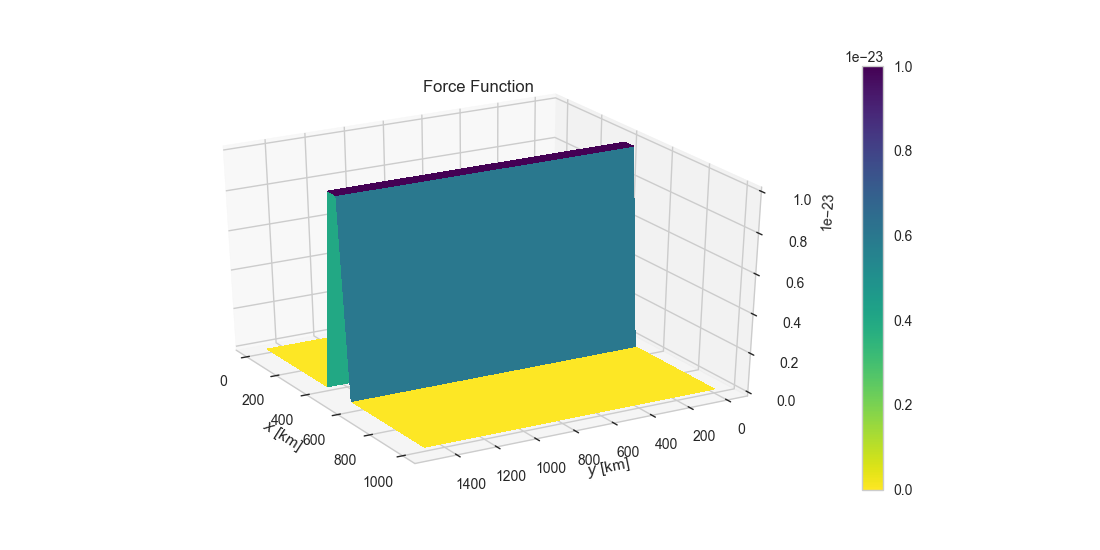
\includegraphics[width=0.4\linewidth]{../Python/output/fd_solution/plots/force_function}
	}
	\subfigure[]{
	    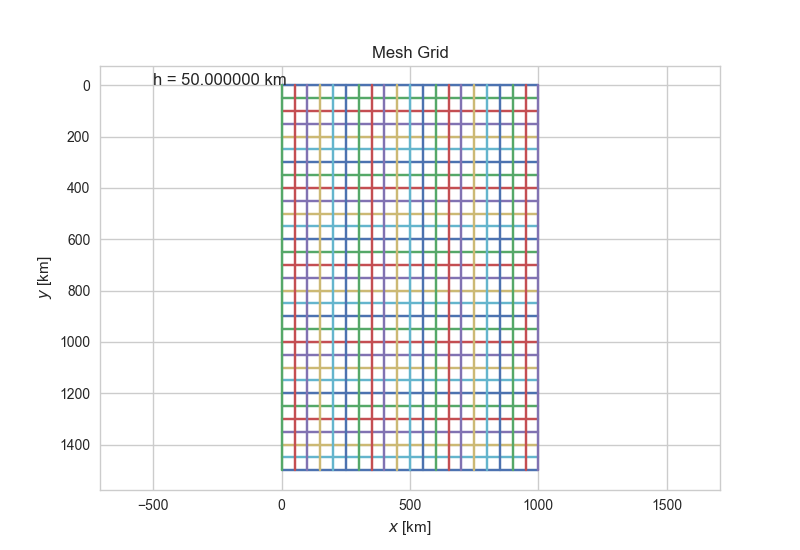
\includegraphics[width=0.4\linewidth]{../Python/output/fd_solution/plots/mesh_grid}
	}
	\caption{The discretized force function (a) and the mesh on which it was computed (b). The computation was done on a regular grid of $21\times31$ nodes, with $g_y=10\ m/s^2$, $\eta=10^{21}\ Pa\cdot{s}$, $3200\ kg/m^3$ and $3300\ kg/m^3$ for the left and right layers.}
	\label{fig:forcefunction}
\end{figure*}

\subsubsection{The finite difference approach}

A finite difference representation of the stream function - vorticity formulation can be obtained by using the same strategy as Eq.\ (3.20), Section 3 of \citet{gerya2009introduction}:
\end{multicols}
\begin{align*}
    \dfrac{\omega_{i,j-1}-2\omega_{i,j}+\omega_{i,j+1}}{\Delta{x}^2} + \dfrac{\omega_{i-1,j}-2\omega_{i,j}+\omega_{i+1,j}}{\Delta{y}^2} &= \dfrac{g_y}{\eta}\dfrac{\rho_{i,j+1}-\rho_{i,j-1}}{2\Delta{x}}, \\
    \dfrac{\psi_{i,j-1}-2\psi_{i,j}+\psi_{i,j+1}}{\Delta{x}^2} + \dfrac{\psi_{i-1,j}-2\psi_{i,j}+\psi_{i+1,j}}{\Delta{y}^2} &= \omega_{ij}.
\end{align*}
\begin{multicols}{2}
where the convention that index $j$ corresponds to the $x$-axis and index $i$ corresponds to the $y$-axis is adopted.

The global index is calculated based on geometrical indices as
\begin{equation}
    k = N_y\times(j-1)+i,
\end{equation}

For both the finite element and the finite difference approaches, after obtaining the solution of the second equation, the stream function will be converted into velocity field based on Eqn.\ (\ref{eq:streamfunction}) using a central difference approach:
\begin{align*}
    v_{x(i,j)} &= \dfrac{\psi_{i+1,j}-\psi_{i-1,j}}{2\Delta{y}}, \\
    v_{y(i,j)} &= -\dfrac{\psi_{i,j+1}-\psi_{i,j-1}}{2\Delta{x}}.
\end{align*}

The velocity components should be computed only on the internal nodes of the grid.

~\\

\section{Results and Discussions}

\subsection{The Navier-Stokes equation}

\subsubsection{Default settings}

We start with a simple problem as described below: the study region is defined by a rectangular box as $[0,1000000]\times[0,1500000]$ and discretized into $20\times30$ blocks horizontally and vertically. A constant, horizontal velocity of $0.8\times10^{-7}$ m/s flowing to the positive $x$-direction were added to the top of the study region. The other three boundaries were constraint by no-slip ($v=0$ m/s) conditions. The density of the fluid is fixed at 3250 kg/m$^3$. The gravity field was ignored. The viscosity is chosen as $10^{21}$ Pa$\cdot$s which is the typical value in the Earth's mantle.

\begin{figure*}[!htb]
	\centering
	\subfigure[]{
		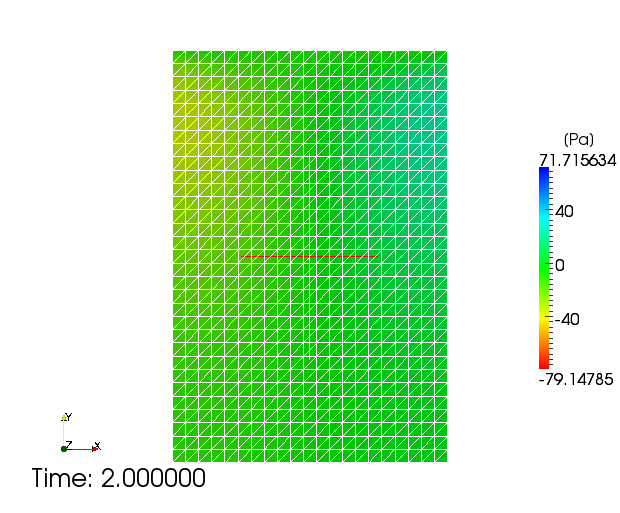
\includegraphics[width=0.4\linewidth]{../Python/report/ns_routine/default_p_2sec}
	}
	\subfigure[]{
		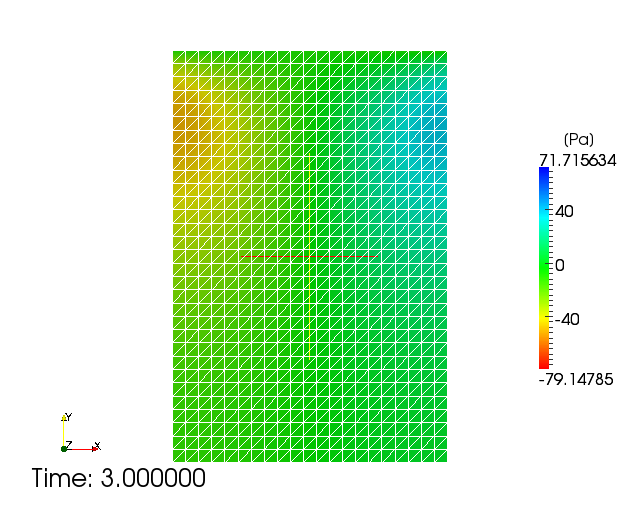
\includegraphics[width=0.4\linewidth]{../Python/report/ns_routine/default_p_3sec}
	}
	\subfigure[]{
		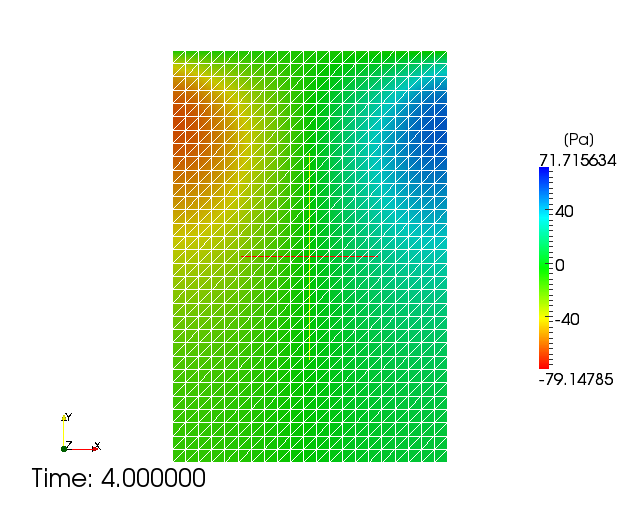
\includegraphics[width=0.4\linewidth]{../Python/report/ns_routine/default_p_4sec}
	}
	\subfigure[]{
		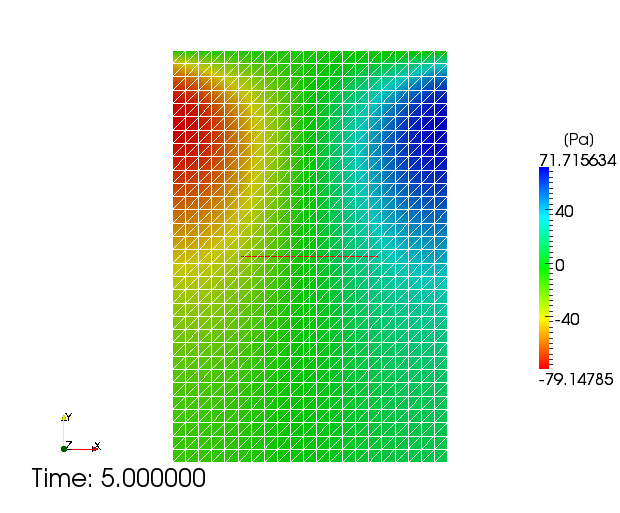
\includegraphics[width=0.4\linewidth]{../Python/report/ns_routine/default_p_5sec}
	}
	\caption{Selected snapshots from the time evolution animation of pressure at time levels 2.0, 3.0, 4.0 and 5.0 sec: high and low pressures are shown in the upper-right and upper-left corners because of the applied velocity boundary condtion.}
	\label{fig:defaultpressure}
\end{figure*}

A few selected snapshots from the time evolution of pressure (Fig.\ \ref{fig:defaultpressure}) show that because of the applied velocity boundary condition, the pressure in the upper-right corner gradually increases to about $72$ Pa. In contrast, the pressure in the upper-left corner dreceases to $-79$ Pa. The magnitude of the maximum velocity in the flow is comparable to the velocity boundary condition, $0.9\times10^{-7}$ m/s (Fig.\ \ref{fig:defaultvelocity}). The zero velocities occur in the center and the two lower corners of the study region. At these places, the fluid remains steady.

\begin{figure}[H]
	\centering
	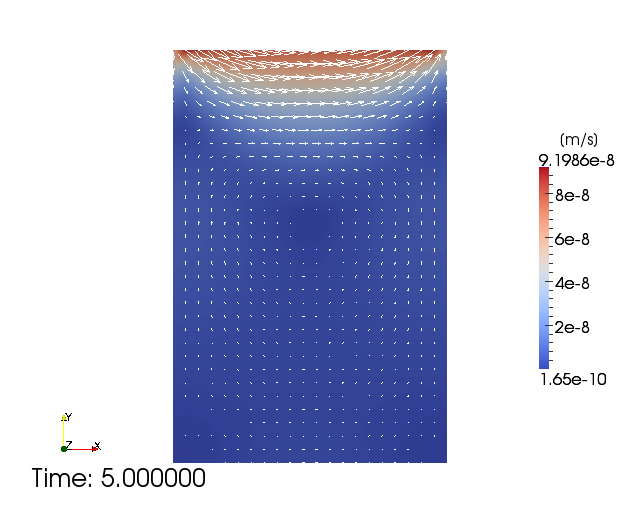
\includegraphics[width=0.7\linewidth]{../Python/report/ns_routine/default_u_final}
	\caption{Steady state of the velocity field: the velocity ranges from 0.01 to 9.62 m/s and low values occur in the center and the two lower corners. The viscosity is chosen as $10^{21}$ Pa$\cdot$s which is the typical value in the Earth's mantle.}
	\label{fig:defaultvelocity}
\end{figure}

By changing the values of velocity at the open edge at the top, we can examine the behavior of the maximum velocity in the steady-state fluid due to the boundary conditon changes, and plot it as a function of the input (Fig.\ \ref{fig:velocity}). The plot shows that the magnitude changes linearly as the velocity at the open edge increases.

\begin{figure}[H]
	\centering
	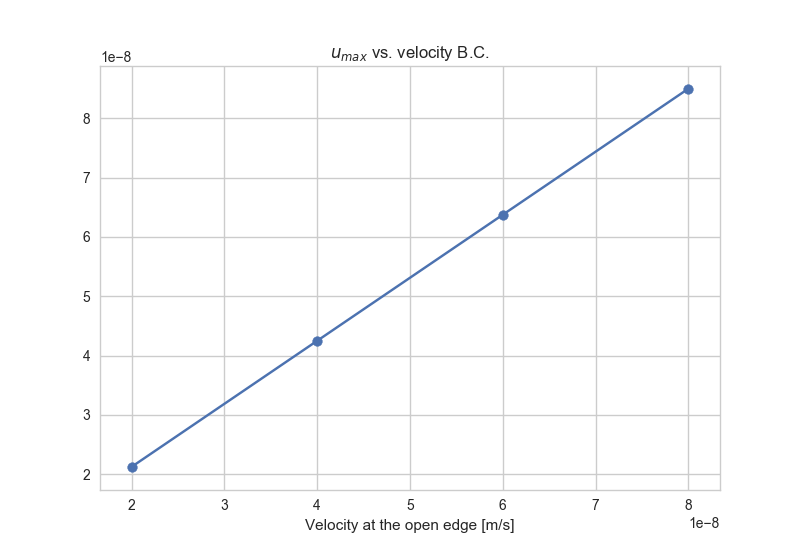
\includegraphics[width=0.7\linewidth]{../Python/output/ns_solution/log/velocity}
	\caption{Maximum velocity in the steady-state fluid as a function of the boundary condition. The magnitude changes linearly with the velocity at the open edge.}
	\label{fig:velocity}
\end{figure}

\subsubsection{More boundary conditions}

Some experiments can be done by using more complicated boundary conditions: an additional velocity boundary condition can be added at the bottom of the study region, with the same magnitude and direction. The flow pattern may differs for different fluids because of their different Reynold's numbers. In this project, behaviors of the matters with significantly different viscosities were studied, as shown in Fig.\ \ref{fig:materials}. The viscosity of granite is in the scale of $10^{19}$. In order to bridge the gap, three imaginary materials with viscosities $2.3\times10^{13}$, $2.3\times10^{11}$, and $2.3\times10^{8}$ Pa$\cdot$s were created.

\begin{figure*}[!htb]
	\centering
	\includegraphics[width=0.7\linewidth]{../Python/report/ns_test/lst_of_materials}
	\caption{A section of the source code in the project, showing the materials being studied. The densities and viscosities are given in the units of kg/m$^3$ and Pa$\cdot$s, respectively. Three imaginary materials with viscosities $2.3\times10^{13}$, $2.3\times10^{11}$, and $2.3\times10^{8}$ Pa$\cdot$s were created to bridge the gap between granite and the other common fluids.}
	\label{fig:materials}
\end{figure*}

Density and viscosity are critical parameters determining the flow patterns, which can be easily seen from the definition of Reynold's number:
\begin{equation}\label{eq:reynolds}
	Re = \dfrac{\rho\bar{u}L}{\mu}
\end{equation}
where $\mu$ is the \emph{dynamic viscosity} in Pa$\cdot$s. To simply the calculation, the average velocity $\bar{u}$ was estimated by multiplying the maximum velocity with a factor of $0.5$.

As expected, the addition of the B.C.\ at the bottom, along with the existing B.C.\ at the top created two vortexes: the one at the top flows clockwisely and the one at the bottom flows counter-clockwisely. However, the pattern cannot be produced when changing the properties of the fluid. A first experiment shows that when reducing the viscosity, the pattern gradually disappeared (Fig.\ \ref{fig:vortexone}). As the viscosity decreases from the $10^{19}$ level to the $10^{13}$ level, there is some slight changes in the flow pattern: the centers of the vortexes became closer to the top the the bottom. As the viscosity dropped to about $10^8$ Pa$\cdot$s and lower, the pattern disappeared.

\begin{figure*}[!htb]
	\centering
	\subfigure[]{
		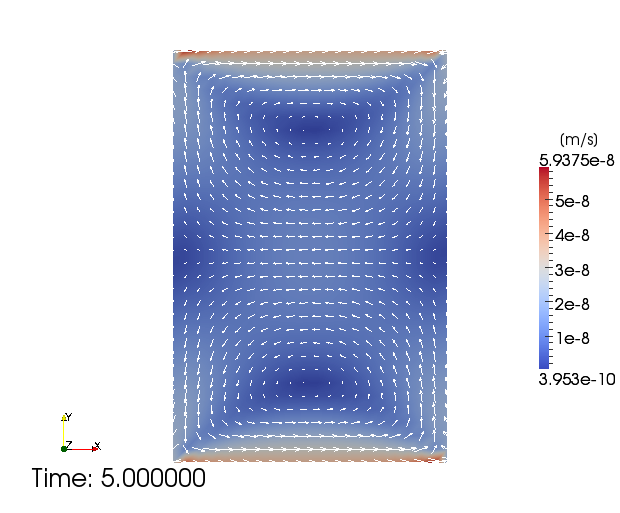
\includegraphics[width=0.4\linewidth]{../Python/report/ns_test/granite_u_final}
	}
	\subfigure[]{
		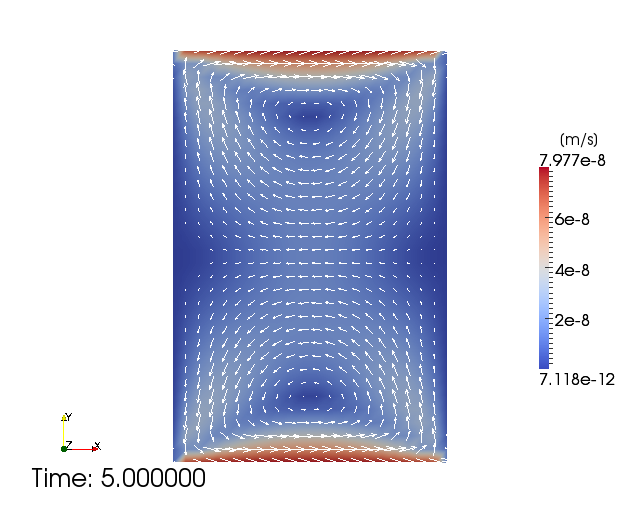
\includegraphics[width=0.4\linewidth]{../Python/report/ns_test/dummy_1_u_final}
	}
	\subfigure[]{
		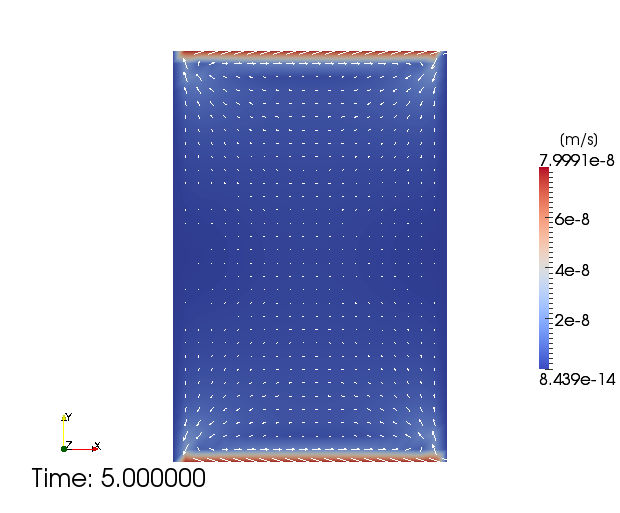
\includegraphics[width=0.4\linewidth]{../Python/report/ns_test/dummy_2_u_final}
	}
	\subfigure[]{
		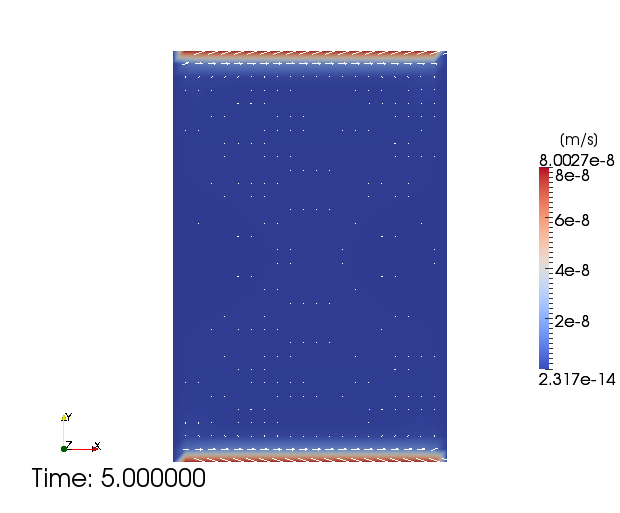
\includegraphics[width=0.4\linewidth]{../Python/report/ns_test/dummy_3_u_final}
	}
	\caption{Final states of the velocity field using different densities and viscosities: (a) granite; (b) imaginary material one; (c) imaginary material two; (d) imaginary material three. The velocity added at the bottom has the same magnitude and direction as the B.C.\ at the top.}
	\label{fig:vortexone}
\end{figure*}

However, another possible reason for the above observation is that the time selected for the animations were not long enough. To exclude this factor, a second test was done by using lengths of 5.0 sec, 50 sec, 500 sec and 5000 sec, respectively (Fig.\ \ref{fig:vortextwo}). The materials being used and all the other parameters remained the same. In the revised test, the flow patterns showed up for all cases after a period of time. However, the reduction of viscosity still exerted some effects on the looks of the patterns.

\begin{figure*}[!htb]
	\centering
	\subfigure[]{
		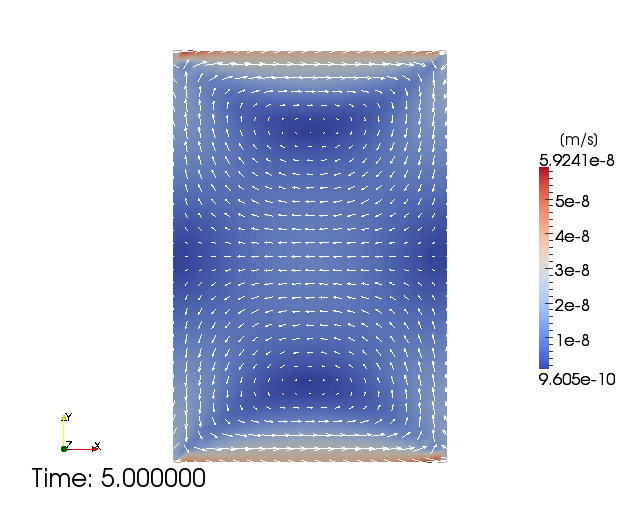
\includegraphics[width=0.4\linewidth]{../Python/report/ns_test/longer_granite_u_final}
	}
	\subfigure[]{
		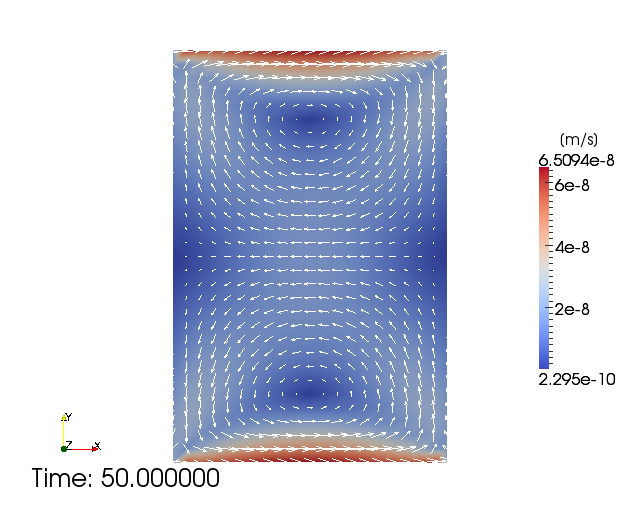
\includegraphics[width=0.4\linewidth]{../Python/report/ns_test/longer_dummy_1_u_final}
	}
	\subfigure[]{
		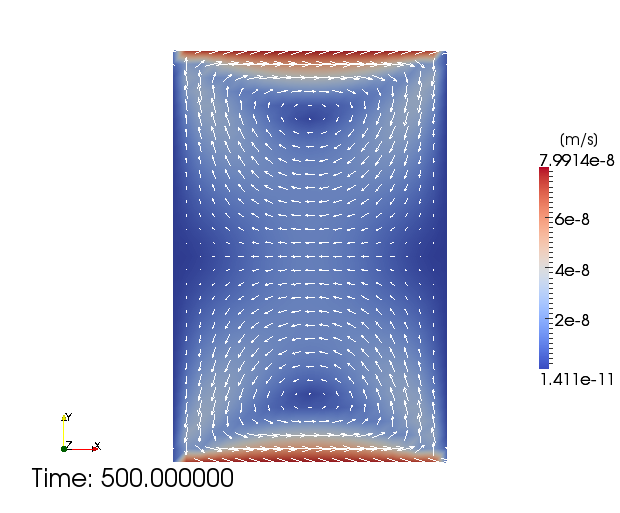
\includegraphics[width=0.4\linewidth]{../Python/report/ns_test/longer_dummy_2_u_final}
	}
	\subfigure[]{
		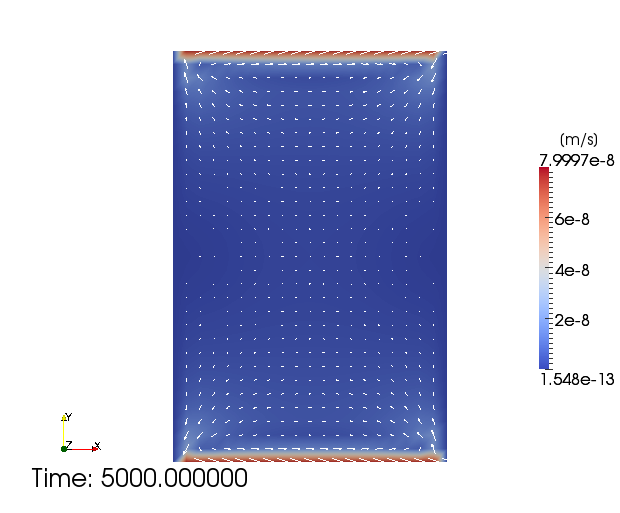
\includegraphics[width=0.4\linewidth]{../Python/report/ns_test/longer_dummy_3_u_final}
	}
	\caption{The same experiment as in Fig.\ \ref{fig:vortexone} repeated with larger time lengths. The time used for the four animations were respectively 5.0 sec, 50 sec, 500 sec and 5000 sec. The revised experiment showed that the reduction of viscosity did not stop the transfer of the velocity B.C.\ to the inner part of the fluid, but the flow pattern has changed due to the reduction of viscosity.}
	\label{fig:vortextwo}
\end{figure*}

\subsection{The vorticity formulation}

\subsubsection{Solutions}

With the vorticity and stream function fixed at zeros on the boundaries, the experiment started from $21\times31$ nodes, $g_x=0,g_y=10\ m/s^2$ for the vertical gravity field, $3200\ kg/m^3$ and $3300\ kg/m^3$ for the left and right layers. The model size is $1000\times1500\ km$ and a constant viscosity of $\eta=10^{21}\ Pa\cdot{s}$ was used. The finite element and finite difference approaches basically produced the same result, as shown in Fig.\ \ref{fig:solutions}. The magnitude of velocities range from $0.0$ to $0.4\times10^{-7}$ km/s in the clockwise flow. Zero velocities basically occurred at the center and the four corners of the study region.

\begin{figure*}[!htb]
	\centering
	\subfigure[]{
		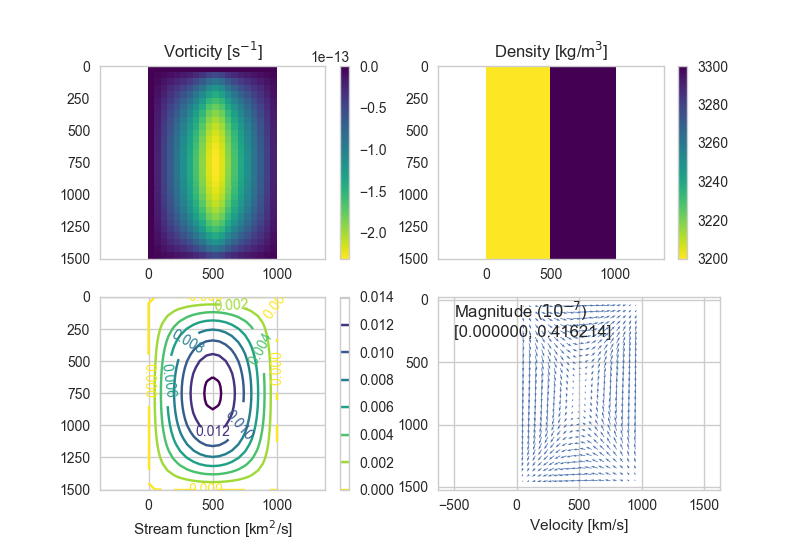
\includegraphics[width=0.9\linewidth]{../Python/output/fe_solution/plots/default}
	}
	\subfigure[]{
		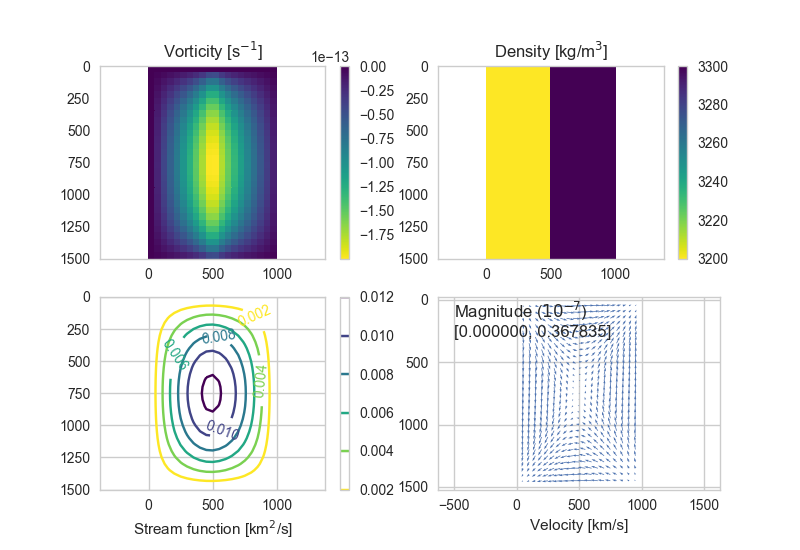
\includegraphics[width=0.9\linewidth]{../Python/output/fd_solution/plots/default}
	}
	\caption{The finite element (a) and the finite difference (b) solutions to the 2-D buoyancy driven flow problem: velocities range from $0.0$ to $0.37\times10^{-7}$ km/s in the resultant clockwise flow; the zero velocities occurred at the center and the four corners of the study region.}
	\label{fig:solutions}
\end{figure*}

For both methods, different spacing and parameters were tried to investigate the accuracy and stability for comparison. The maximum magnitudes of the velocity field were plotted as functions of input parmeters (Fig.\ \ref{fig:fevsfd}). The experiment showed that the maximum magnitude of the velocity field increased linearly as the gravity and the density contrast between the two layers increased, but showed an inverse relationship with the viscosity of the fluid. The finite element and finite difference solutions showed a tiny difference. Different from the pipe flow problem for which an analytic solution can be found, without an exact solution to the buoyancy driven flow, one cannot say anything about the accuracy of the two methods in this study. Having the suspect that the grid size could have exerted an effect on the accuracy of the solutions, the grid number was increased from $21\times31$ to $41\times31$ for both methods. Completely no reduction in the discrepancy was observed.

\begin{figure*}[!htb]
	\centering
	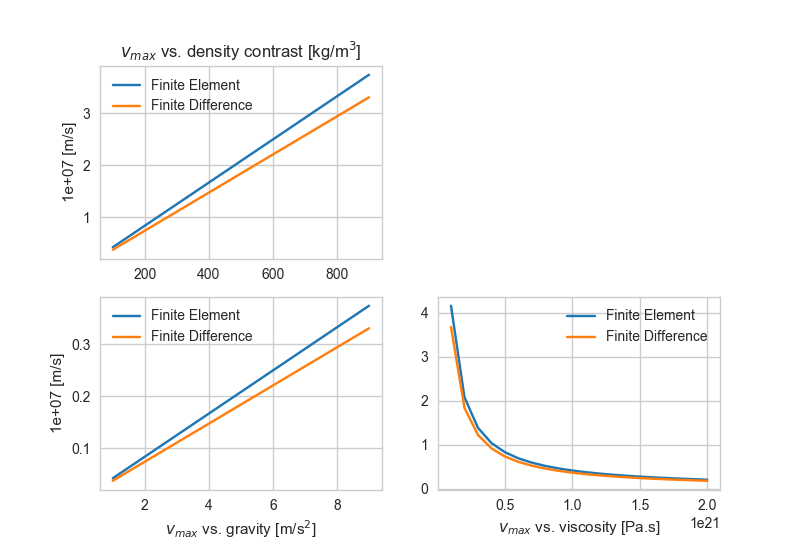
\includegraphics[width=0.7\linewidth]{../Python/output/fd_solution/log/fe_vs_fd}
	\caption{Maximum magnitudes of the velocity field as functions of gravity, density contrast between the two layers and viscosity: blue curves, solutions using the finite element approach; orange curves, solutions using the finite difference approach.}
	\label{fig:fevsfd}
\end{figure*}

\subsubsection{Performance test}

The FeniCS project implicitly uses just-in-time (JIT) compilation to solve finite element problems. The finite element codes for this project run very fastly. Nevertheless, the finite difference code for the stream function approach was written in Python and is not as efficient as the finite element codes. Therefore, we came up with the idea of accelerating the code using Numba.

A section of codes was selected to do the performance test (Fig.\ \ref{fig:performtest}). The code calls \textsf{stream\_2d()} to repeatedly solve the 2D stream function problem with different input parameters. The performance test showed that without using Numba, the code took 58.416270 sec to execute; while after accelerating the subroutine \textsf{stream\_2d()}, it took 51.385716 sec to execute.

\begin{figure*}[!htb]
	\centering
	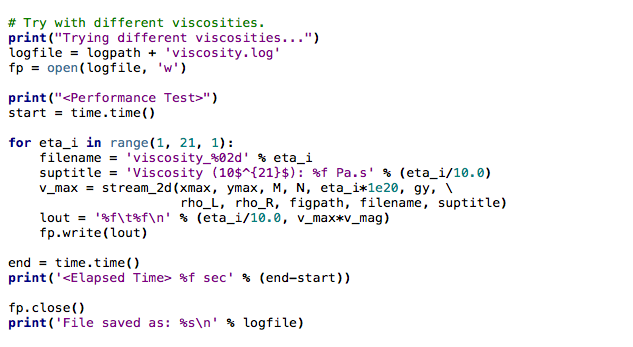
\includegraphics[width=0.7\linewidth]{../Python/report/fd_numba/perform_test}
	\caption{A section of codes being used to run the performance test. Timing commands were added before and after the loop.}
	\label{fig:performtest}
\end{figure*}

The first iteration using Numba actually took much longer time to run than ordinary Python, whereas as the execution continued, the later iterations took less time and the acceleration accumulated, which made the total time shorter.

~\\

\section{Conclusions}

\begin{itemize}
	\item{In the first problem, several different velocities were used at the boundary to drive a 2-D incompressible flow, the relationship between the maximum magnitude in the velocity field and the boundary condition is linear. After an additional velocity boundary condition with the same magnitude and direction was added, two vortexes in the flow were observed.}
	\item{Several materials, including imaginary matters, with different viscosities were used to try the experiment. Within the same time period (5 sec), the materials with viscosities $10^{11}$ Pa$\cdot$s and $10^8$ Pa$\cdot$s did not show the expected flow patterns. After the animations were extended to 500 sec and 5000 sec, the flow patterns showed up but are still different from those with viscosities $10^{19}$ Pa$\cdot$s and $10^{13}$ Pa$\cdot$s.}
	\item{In the second problem, different input parameters were tried to solve the same buoyancy driven flow velocity field. The results turned out to be that the maximum magnitude in the velocity field is linearly related to the gravity and density constrast, and inversely related to the viscosity.}
	\item{Acceleration of Numba is significant when there are sufficient number of iterations in the code to compensate the time lose during the first iteration, otherwise, the time spent on the first iteration makes Numba slower than ordinary Python.}
	\item{The solutions given by the finite element and finite difference approaches are consistent. There are some slight differences between the solutions of the two methods, but an exact solution is needed for comparison in order to figure out which method is more accurate. No reduction in the discrepancy was observed as the grid number was increased from $21\times31$ to $41\times31$ for both methods.}
\end{itemize}

~\\

\bibliography{references}
\bibliographystyle{apalike}

\end{multicols}

\end{document}
